\documentclass[a4,center,fleqn]{NAR}
\usepackage[pdftex,
colorlinks=true, %makes the links show up in color, rather than in a box
citecolor=black, %color of the in-text citation numbers
urlcolor=blue %color of the url links
]{hyperref}
\usepackage{wrapfig}
\bibliographystyle{unsrt}

% Enter dates of publication
\copyrightyear{}
\pubdate{}
\pubyear{}
\jvolume{}
\jissue{}

\usepackage[usenames,dvipsnames]{color}
\definecolor{red}{rgb}{1,0,0}
\newcommand{\mc}[1]{\textcolor{red}{#1}}

% \articlesubtype{This is the article type (optional)}

% Some shortcuts to make life easier when writing latex
\newcommand{\peace} {{\small PEACE}}
\newcommand{\wcd} {{\small WCD}}
\newcommand{\capthree} {{\small Cap3}}
\newcommand{\easycluster} {{\small EasyCluster}}
\newcommand{\metasim} {{\small MetaSim}}

\begin{document}

\title{PEACE: {\underline P}arallel {\underline E}nvironment for {\underline A}ssembly
  and {\underline C}lustering of Gene {\underline E}xpression}

\author{D.M. Rao\,$^{1}$, J.C. Moler\,$^{1}$, M. Ozden\,$^1$, Y. Zhang\,$^{1}$,
  C. Liang$^{1,2*}$\, and J.E. Karro\,$^{1,3}$\footnote{to whom
    correspondence should be addressed}}

\address{$^1$ Department of Computer Science and Software Engineering, \\
  $^2$ Department of Botany, \\
  $^3$ and Department of Microbiology, Miami University, Oxford, Ohio,
  USA}



\history{Received Feb. 13, 2010 \\ Resubmitted April 20, 2010}

\maketitle

\begin{abstract}
  \mc{We present \peace, a stand alone tool for the high-throughput
    {\it ab initio} clustering of transcript fragment sequences
    produced by Next Generation or Sanger Sequencing technologies,
    freely available from
    \href{http://www.peace-tools.org}{www.peace-tools.org}.  Installed
    and managed through a download-able user-friendly GUI, \peace\/ can
    process large data sets of transcript fragments of length 50 bases
    or greater, grouping the fragments by gene associations with a
    sensitivity compatible to leading clustering tools.  Once
    clustered, the user can employ the GUI's analysis functions,
    allowing the easy collection of statistics and single out specific
    clusters for more comprehensive study or assembly.  Using a novel
    minimum spanning tree based clustering method, \peace is the equal of
    other leading tools in the literature.  It produces results of
    quality virtually identical to those of the \wcd\/ tool when
    applied to Sanger sequences, significantly improved results over
    \wcd when applied the products Next Generate Sequencing
    Technology, and significantly improved results over \capthree in
    both cases.  In short, \peace provides an easily accessible user interface
    for interface with a clustering engine that is the match of the
    leading clustering tools in the literature.}




\end{abstract}


\section{Introduction}

Understanding an organism's transcriptome, the set of (spliced)
transcripts expressed by genes of the organism, is a vital step in
understanding the full functional and organizational role of the
genome in the life cycle of any eukaryote.  Studying the transcriptome
has led to gene discovery, provided information on splice variants,  
and helped shed light on the biological processes both controlling and
controlled by the genome \cite{Nagaraj07}.  However, to access those
transcripts, we must deal with the fragmented data produced by
both Next Generation and traditional Sanger sequencing technology.

In the past, access to a transcriptome sequence was primarily
through the use of Expressed Sequence Tags (ESTs), single-pass cDNA
sequences derived from transcribed mRNAs and sequenced by Sanger
Sequencing technology.  More recently, Next Generation Sequencing
(NGS) technology has begun to rapidly replace Sanger Sequencing,
allowing for more comprehensive coverage of the transcriptome.  For
example, ESTs now being added to the GenBank dbEST are increasingly
the product of NGS technologies such as 454 pyrosequencing, which
enables the sequencing of novel and rare transcripts at a considerably
higher rate of coverage than Sanger Sequencing
\cite{Cheung2006,Emrich2007}.  From a computational perspective, this
is a mixed blessing: while NGS provides immense quantities of new
information, it also provides immensely larger data sets -- and thus a
need for fast, efficient analysis algorithms.

\enlargethispage{-65.1pt}

Given a set of transcript fragments sampled from across the genome, a
necessary first step of the set's analysis is that of clustering: separating
the fragments according to the transcript from which they were
derived.  Frequently performed implicitly by assembly tools,
clustering the data as a ``pre-assembly'' step has a number of
advantages.  Most significantly: performing this step will
allow the application of the assembly tool to individual clusters --
saving significant amounts of time \cite{Hazelhurst08a}.  

However, clustering is a computationally challenging problem.  Even
with the smaller number of ESTs produced using Sanger Sequencing, the
runtime and memory requirements to cluster on the basis of pair-wise
sequence alignments make such an approach infeasible in practice.  The
much larger data-set size produced by NGS technologies exacerbates
this problem.  To deal with this, \peace\/ combines our own version of
the $d^2$ alignment-free sequence distance function \cite{Hide94} and
the concept of a {\it minimum spanning tree} \cite{Prim57} to quickly
and accurately find clusters of ESTs expressed from the same gene
without reference to a sequenced genome.  Compared against \wcd, the
leading clustering tool in the literature \cite{Hazelhurst08a}, as well as
other tools designed for the same purpose 
\cite{Burke99,Slater00,Huang99,Parkinson02,Kalyanaraman03,Malde03,
  Ptitsyn05,Hazelhurst08a,Picardi09}, \peace\/ proves to be both more
sensitive and more robust to sequencing error without sacrificing
runtime.  Nor are any of these tools designed for the ease of installation
and use that \peace\/ provides.

In short, \peace\/ is a computational tool for the {\it ab initio}
clustering of transcript fragments by gene association, applicable to
both NGS and traditional Sanger Sequencing technologies.  Available
through the \href{http://www.peace-tools.org}{www.peace-tools.org}
website, the \peace\/ GUI allows the user to both easily install
(locally or remotely) and run the clustering engine, as well as
enabling transparent parallel processing and providing various tools
for result analysis.

\section{\peace\/: Installation and Use}

The \peace\/ GUI can be launched by downloading and executing the
Jar file available on the \peace\/ website
(\href{http://www.peace-tools.org}{www.peace-tools.org}) to any
machine running the standard Java Virtual Machine (JVM).  Once
running, the user can employ the GUI to install the clustering engine
and perform a clustering of a data file in {\sc fasta} format, view an
initial analysis of the clusters, and produce files containing subsets
of the clusters as input to assembly tools such as \capthree\/ 
\cite{Huang99}.  A typical (first) use of \peace\/ must be
performed in the following manner (see Figure~\ref{fig:workflow}):

\begin{figure}
  \centerline{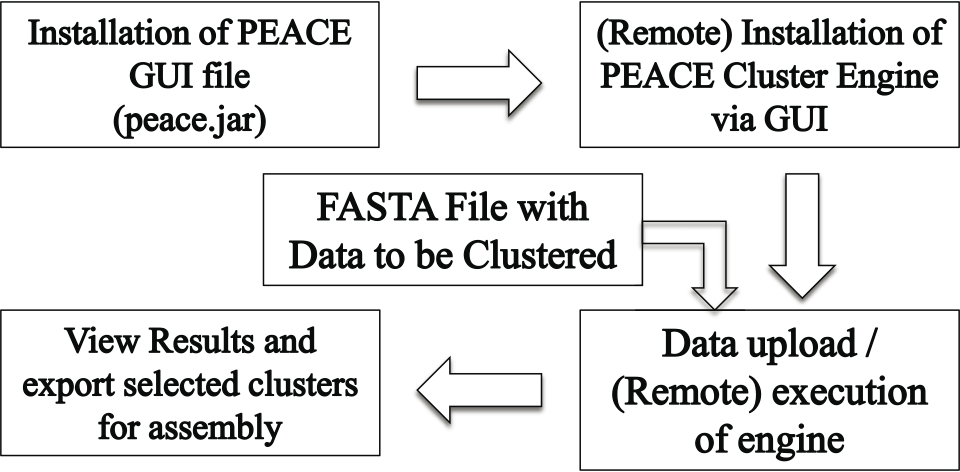
\includegraphics[width=3in]{pics.d/workflow.png}}
  \caption{Overview of the procedure for clustering and analysis using
    PEACE.}\label{fig:workflow}
\end{figure}


\noindent {\bf Tool Installation:} (First use only.) To install the
\peace\/ clustering engine onto a local or remote machine, the user selects
from within the GUI the appropriate menu tab (Figure~\ref{screen}(a)),
which then starts an install wizard that will prompt for the
appropriate information.  Figure~\ref{screen}(b) illustrates the
request for server information; the user has chosen to install the
\peace\/ computational tool on a remote machine and is providing
the necessary connection information.  Server information is
persistent between GUI sessions, giving the user access to \peace\/
on the target machine as needed.

\begin{figure*}
  \begin{minipage}{3in}
    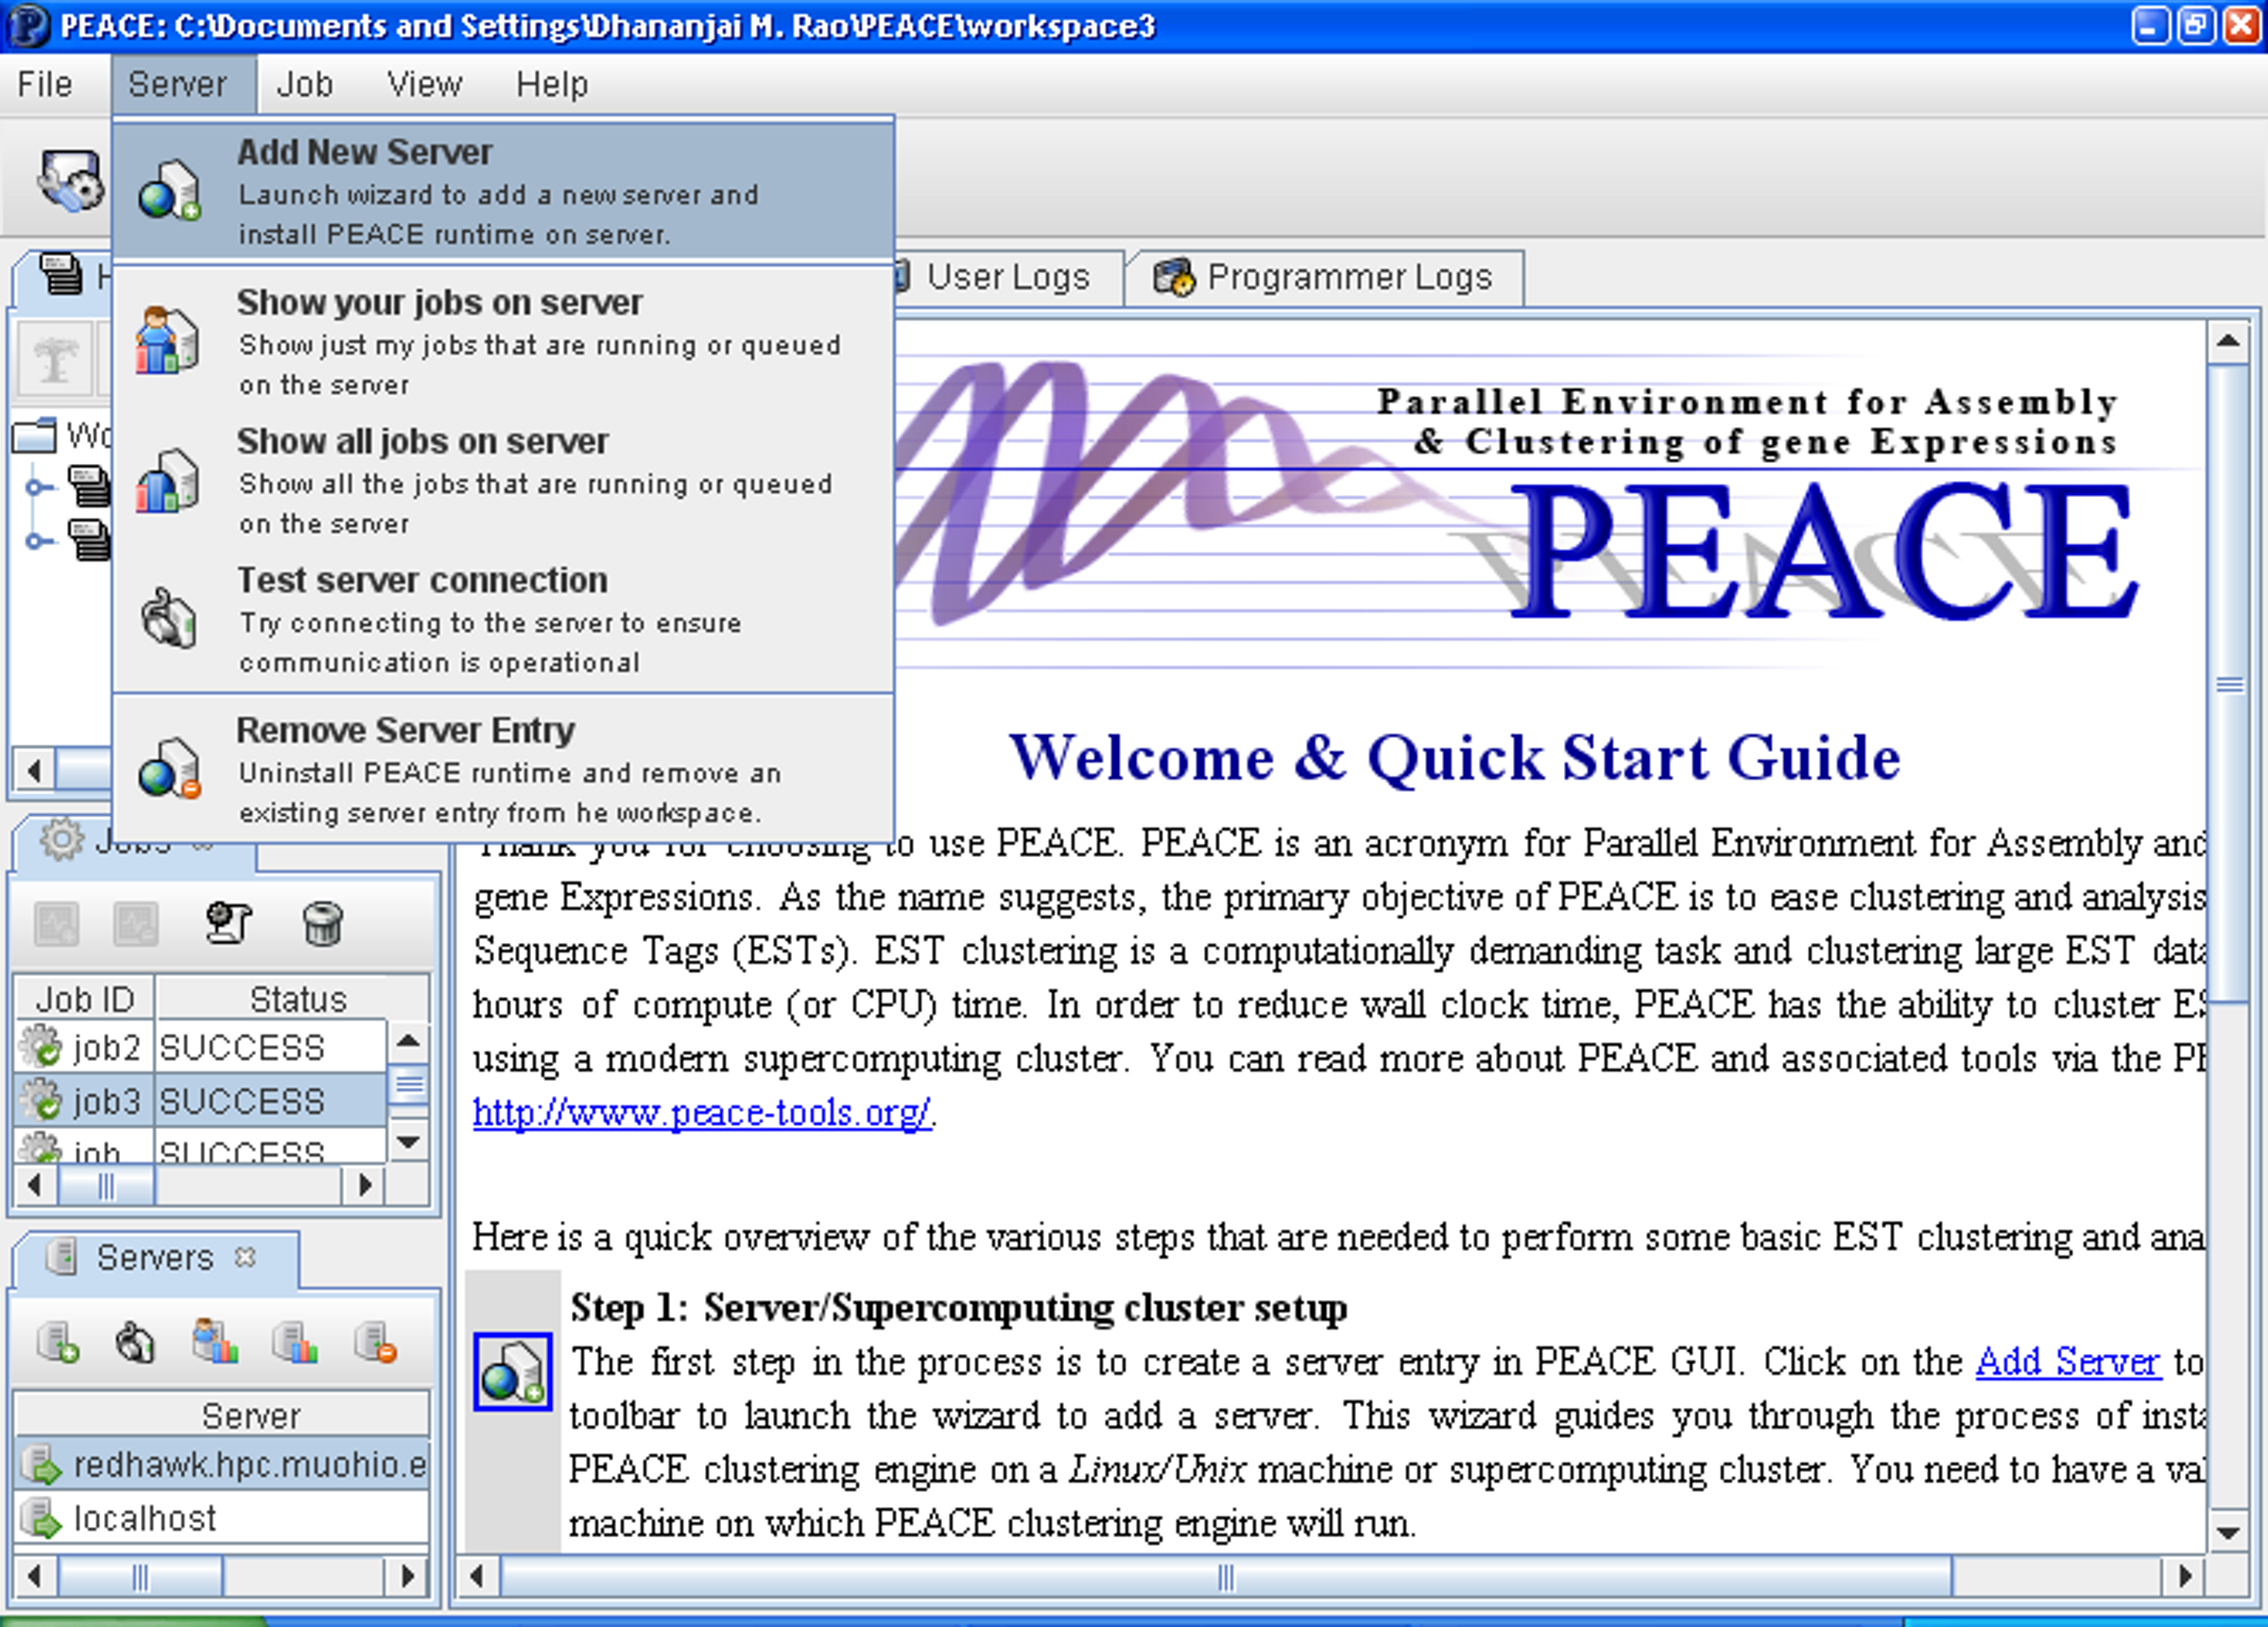
\includegraphics[width=3in]{screen.d/install_page_big.png}
    \centerline{\small{(a)}}
  \end{minipage}
  \begin{minipage}{2in}
    \vspace{0.47in}
    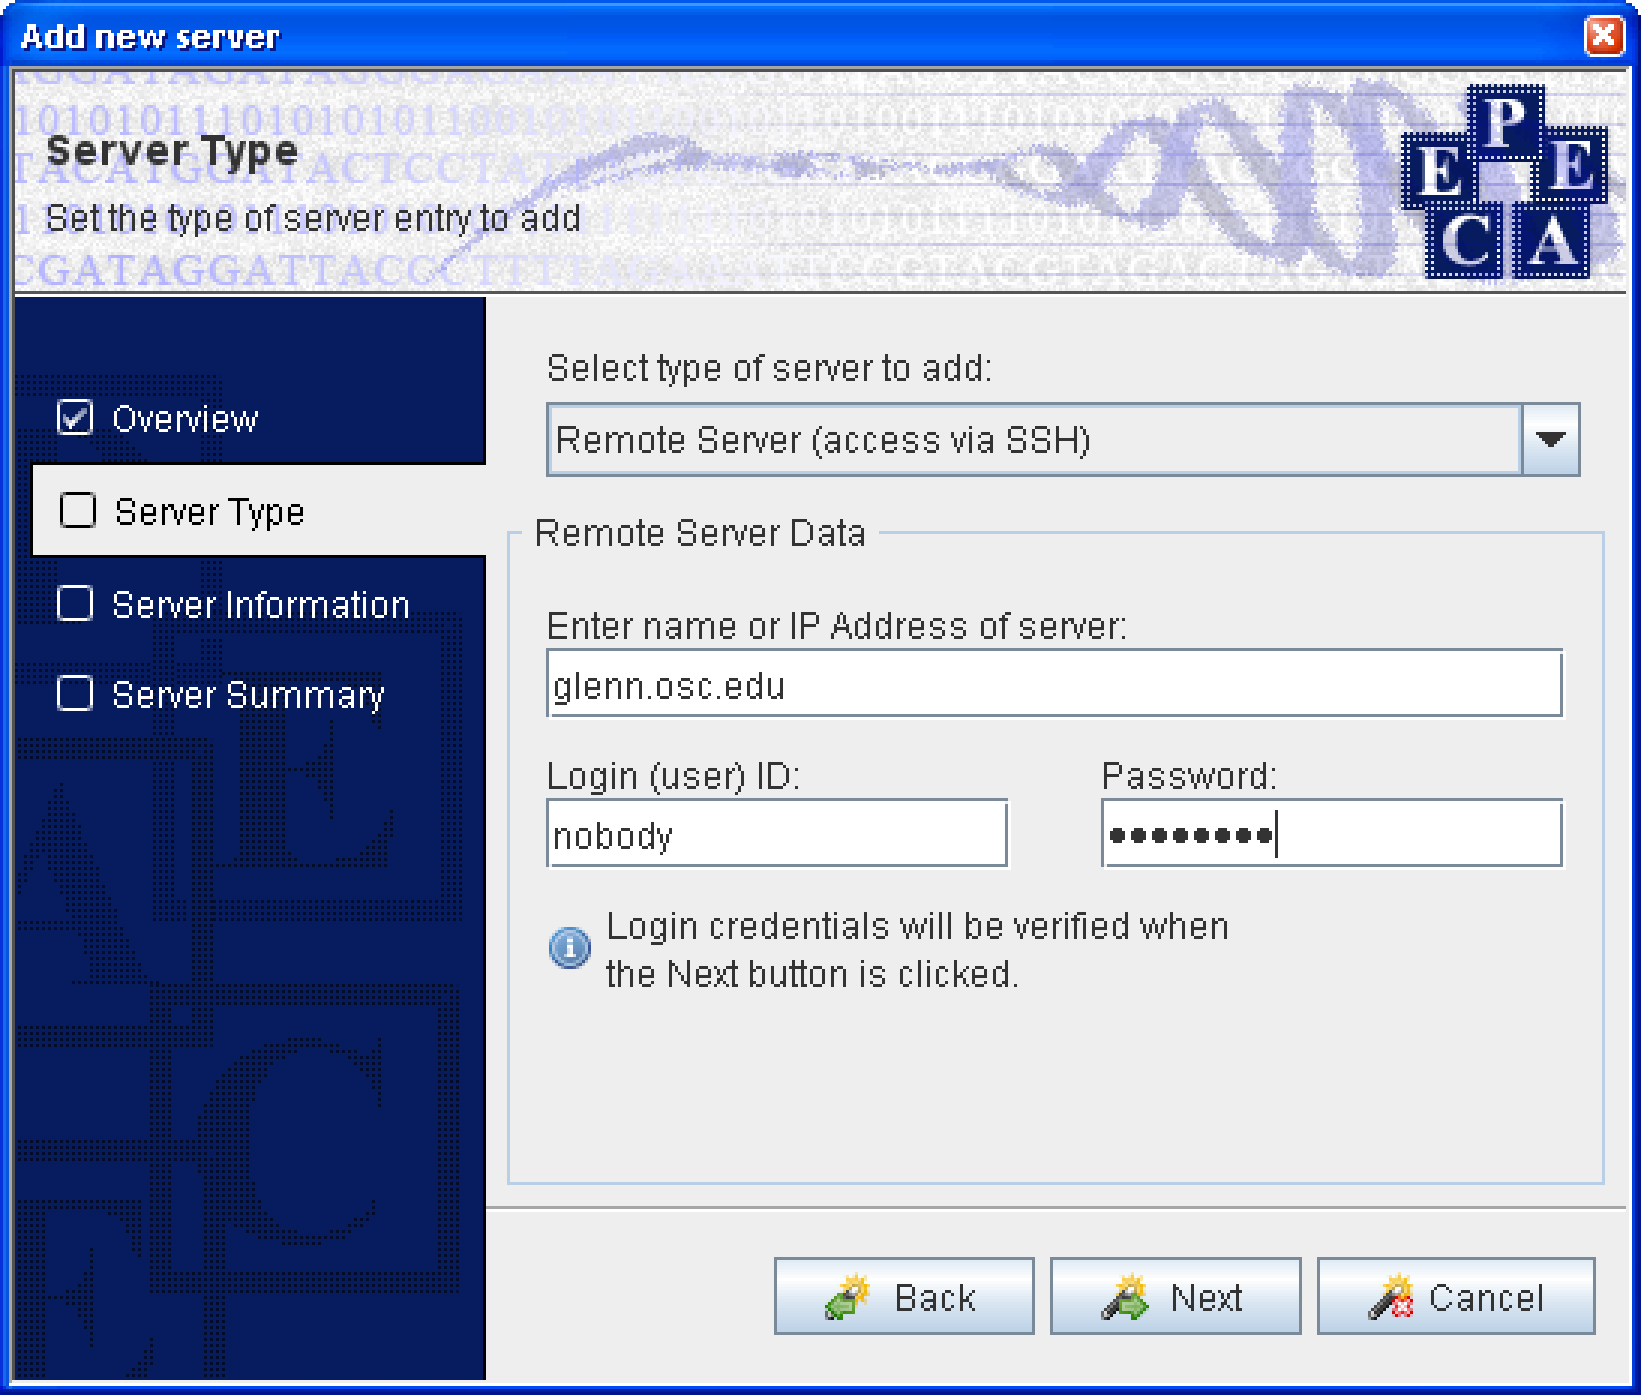
\includegraphics[width=2in]{screen.d/add_server_big.png}
    \centerline{\small{(b)}}
  \end{minipage}
  \begin{minipage}{2in}
    \vspace{0.47in}
    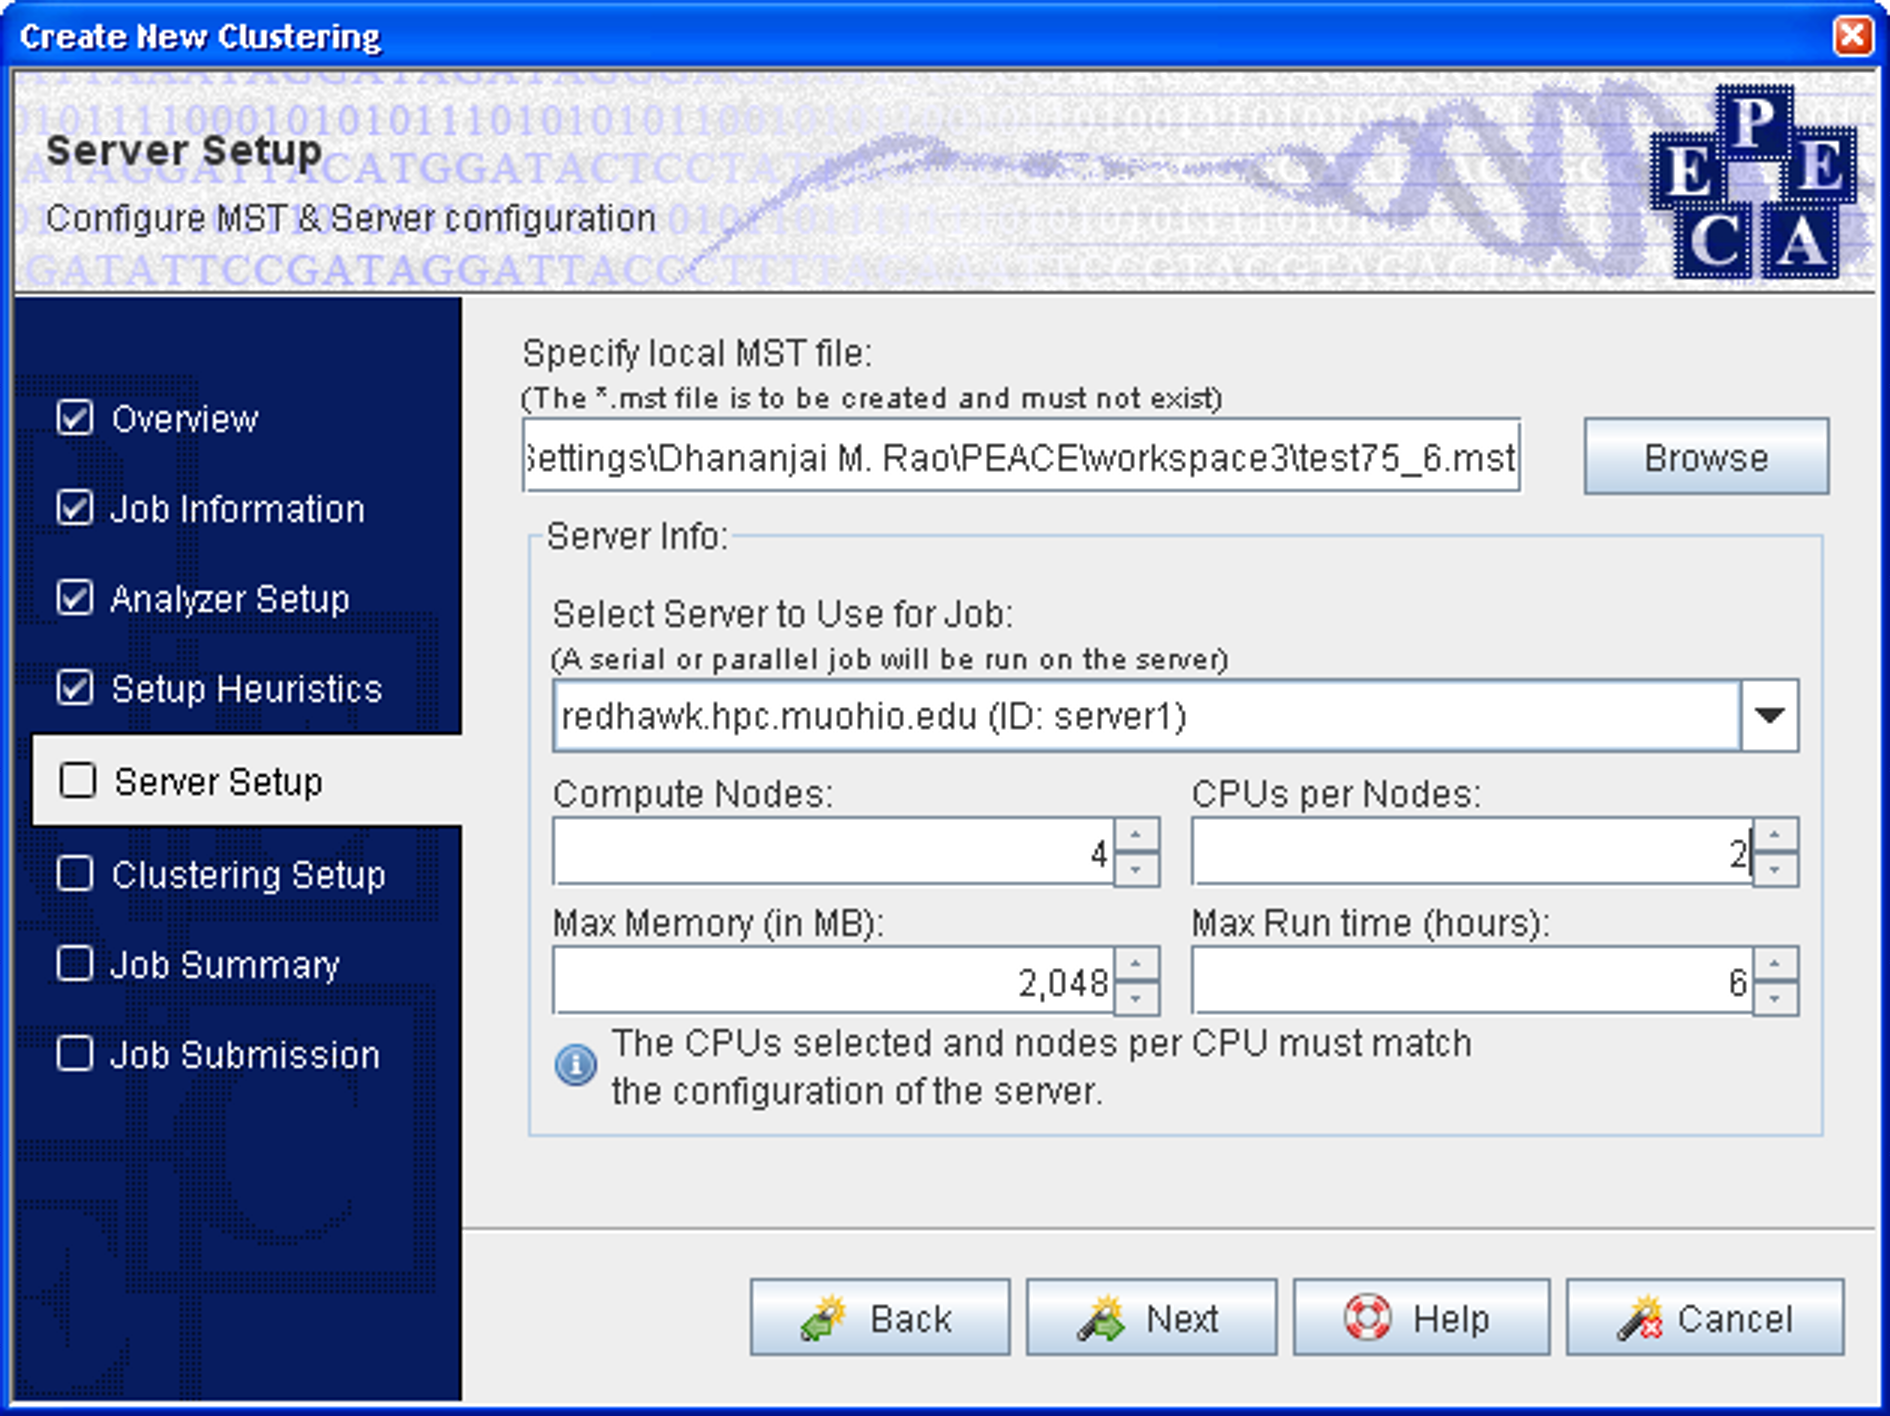
\includegraphics[width=2in]{screen.d/processor_assignment_big.png}
    \centerline{\small{(c)}}
  \end{minipage}

  \begin{minipage}{3in}
    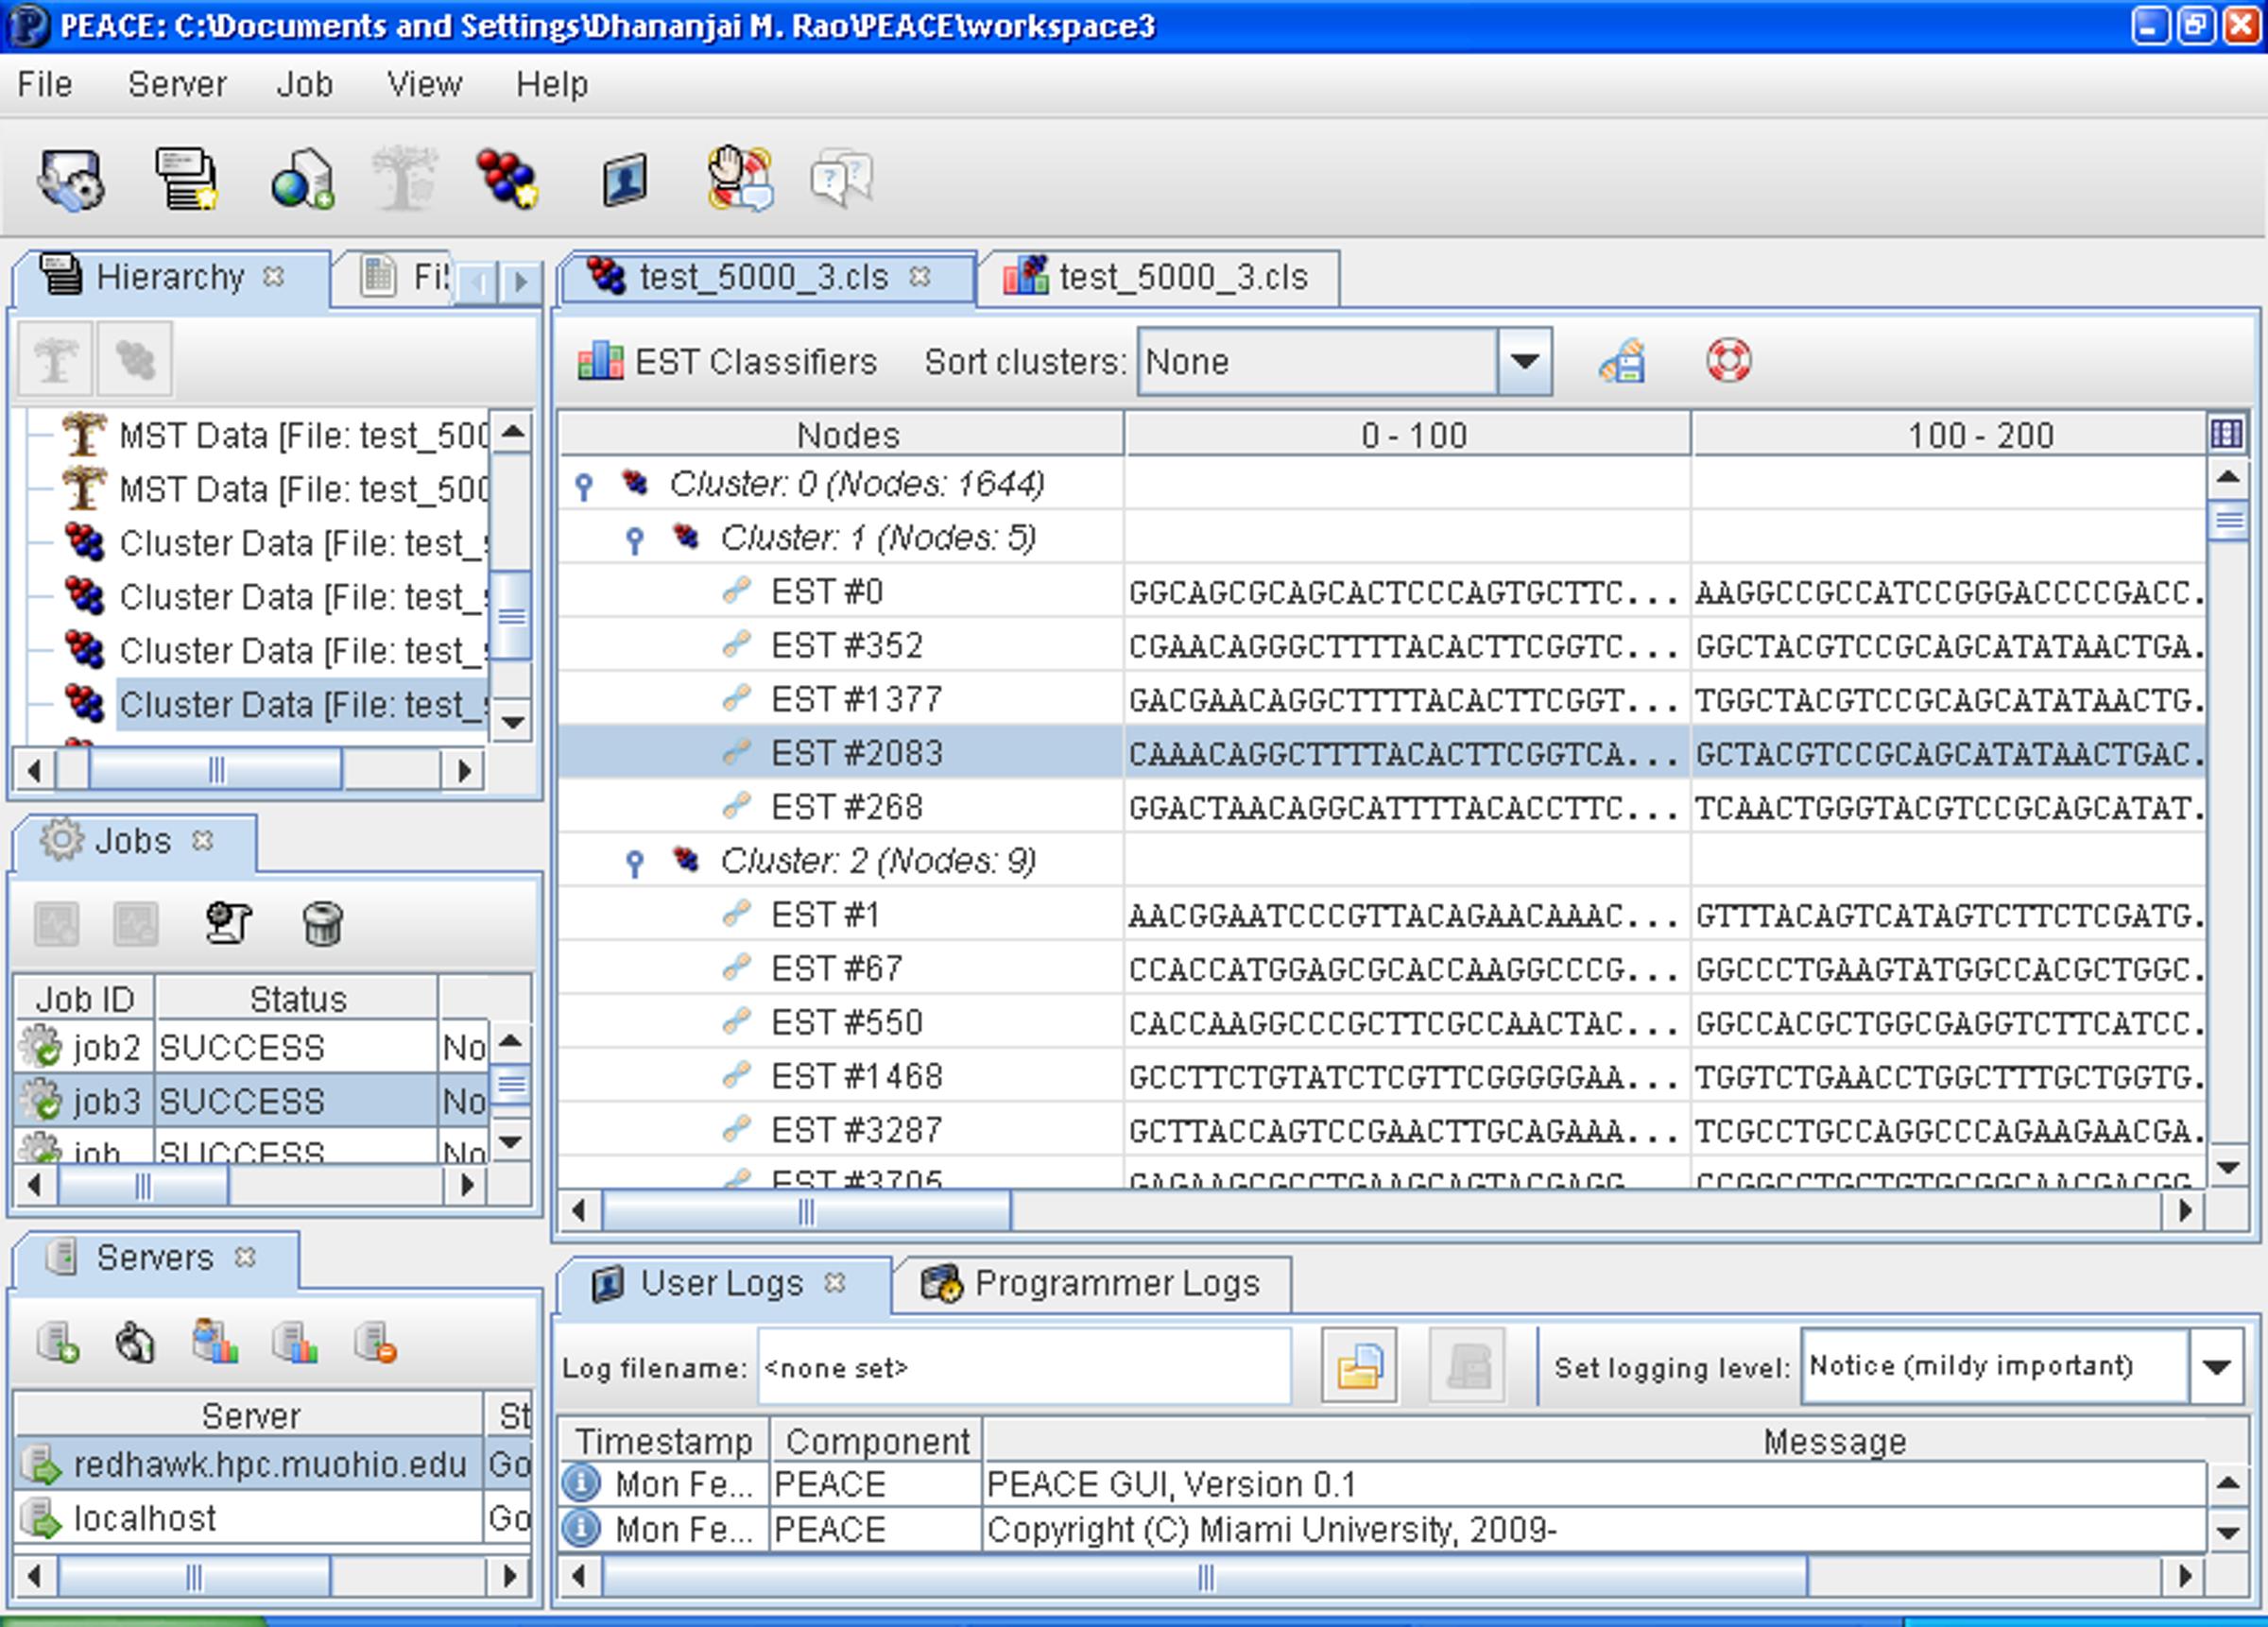
\includegraphics[width=3in]{screen.d/cluster_list_big.png}
    \centerline{\small{(d)}}
  \end{minipage}
  \begin{minipage}{1in}
    \hspace{1in}
  \end{minipage}
  \begin{minipage}{3in}
    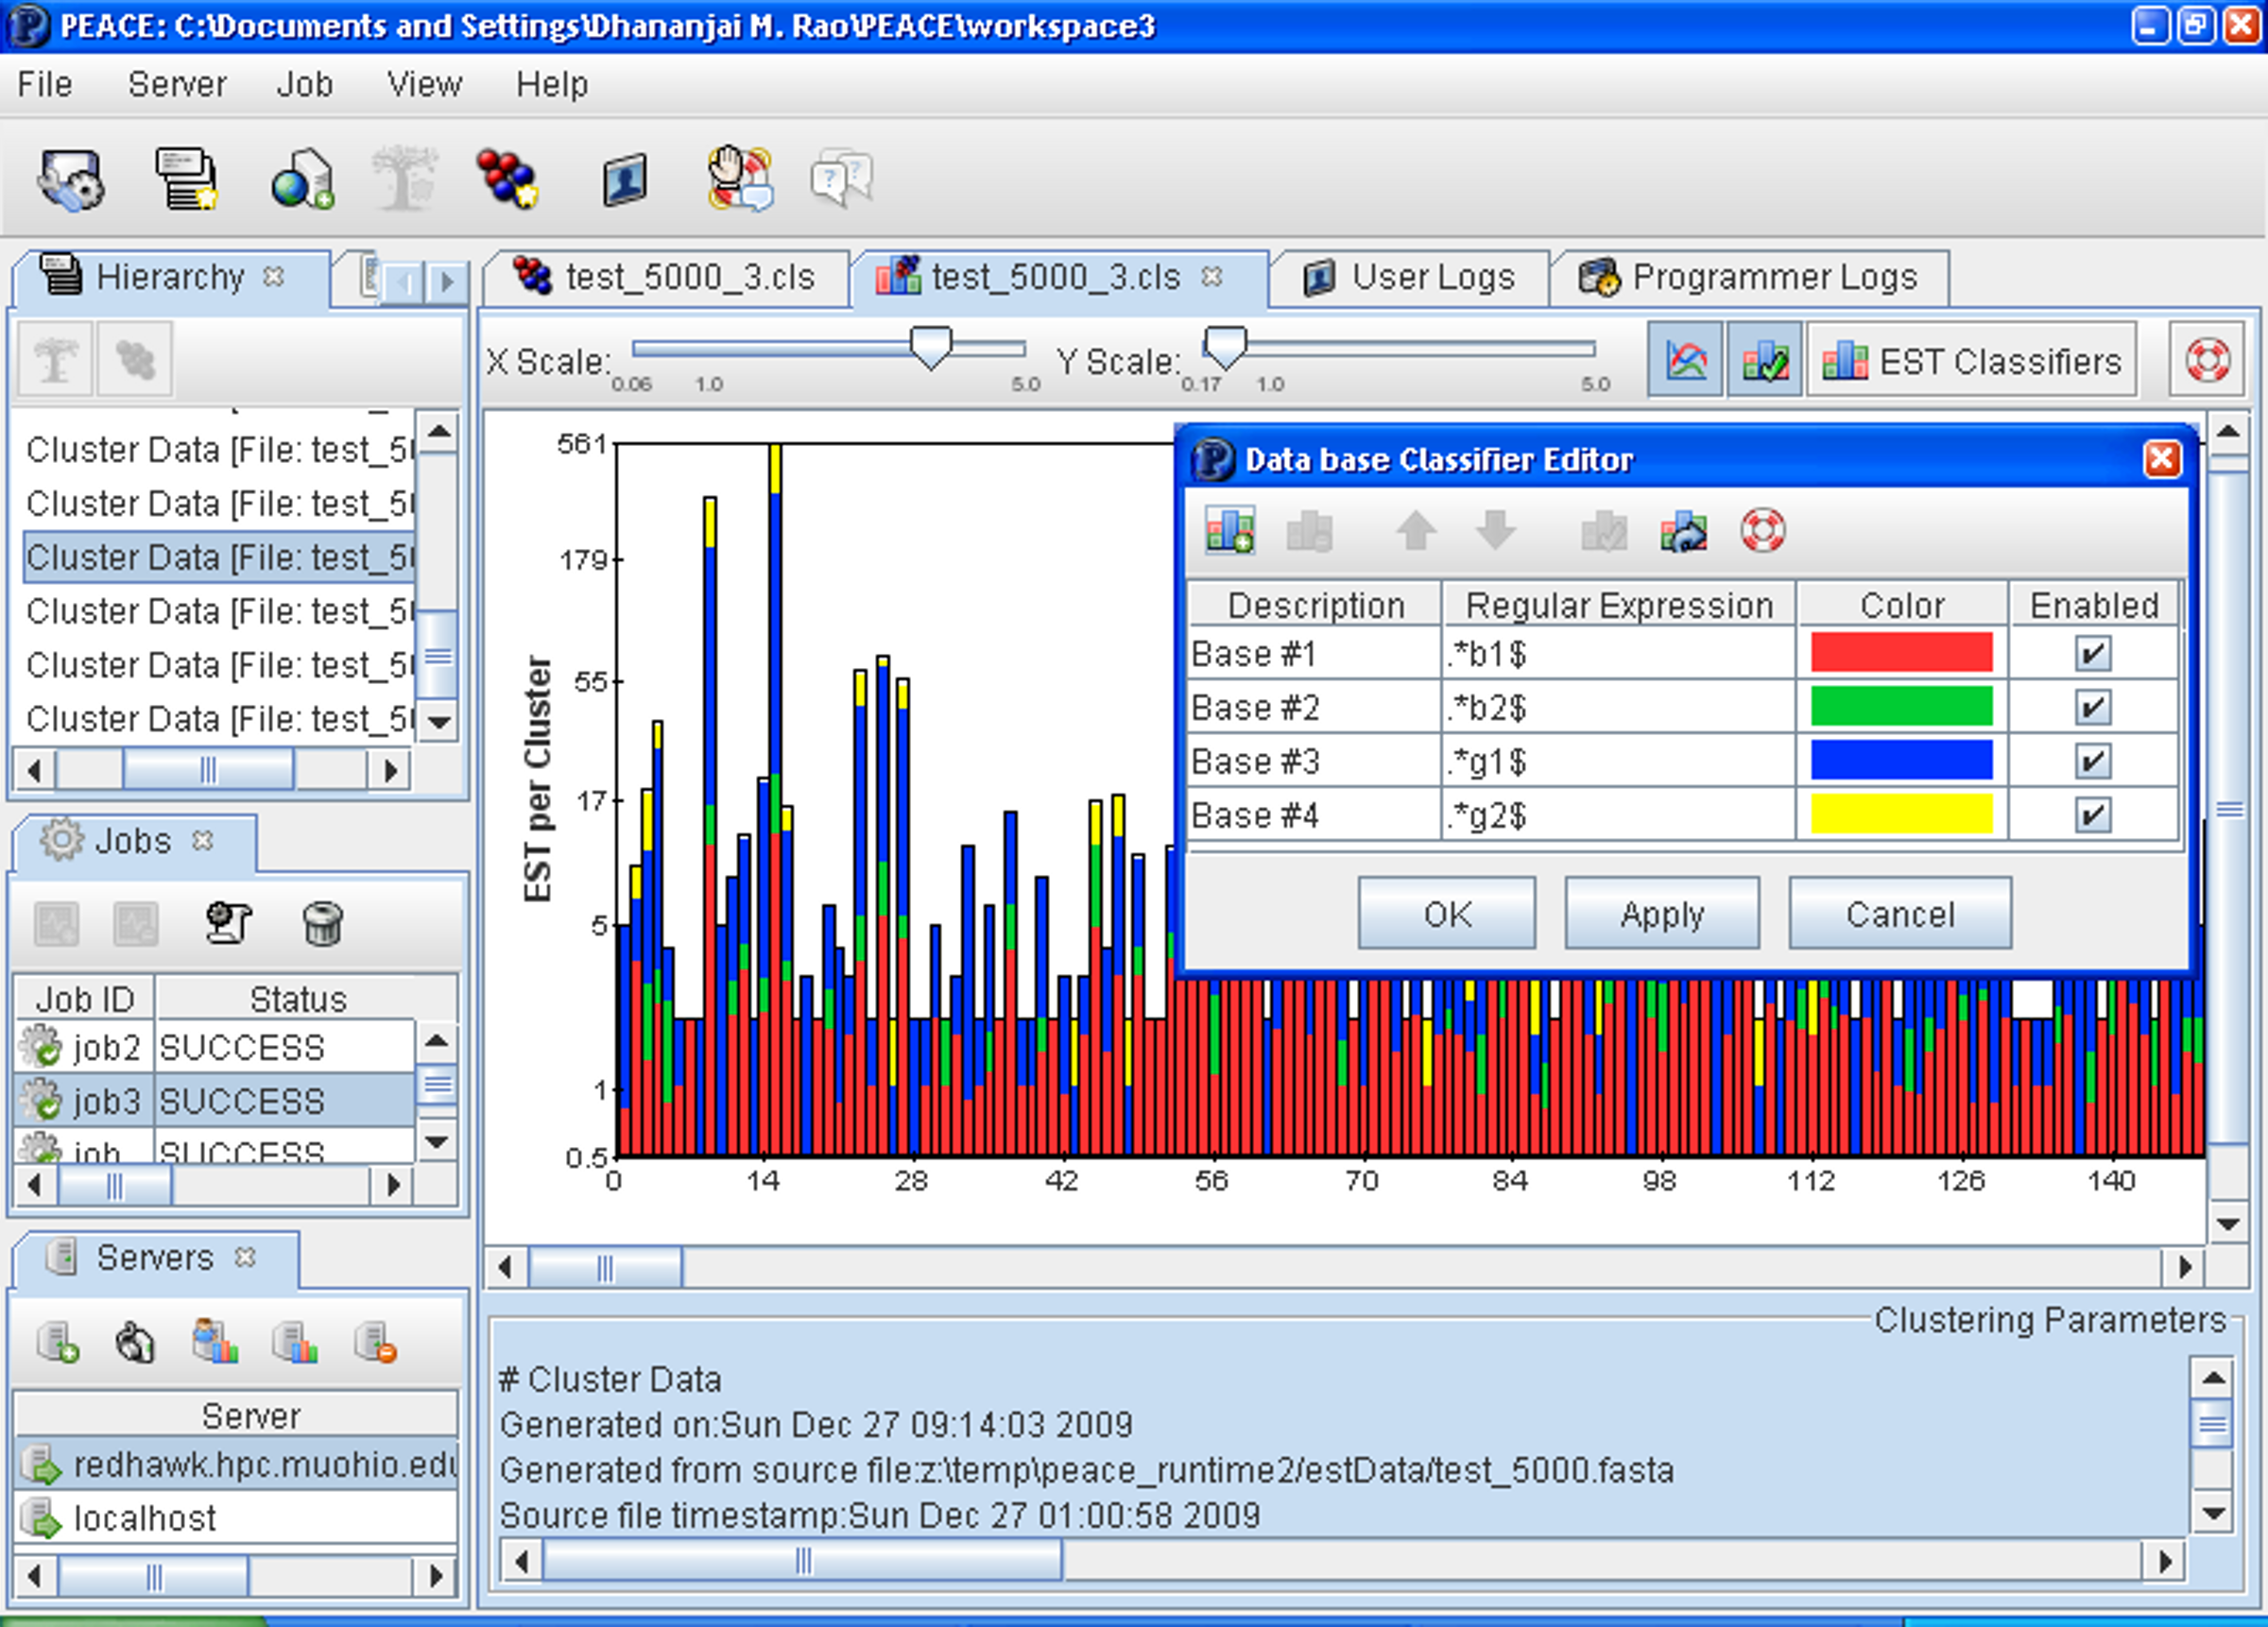
\includegraphics[width=3in]{screen.d/classifier_big.png}
    \centerline{\small{(e)}}
  \end{minipage}

  \caption{Screenshots of the \peace\/ GUI during execution, including (a)
    GUI Welcome and server installation menu; (b) setup wizard for
    installing the computational tool on a remote server; (c) execution
    wizard for starting a selected job to be executed in parallel mode;
    (d) basic cluster output; and (e) histogram view of cluster results
    and classifier editor for setting up differential expression profiles.}\label{screen}
\end{figure*}

\noindent {\bf Job Processing:} After importing the target sequence
file into the GUI, the user starts a new job by following the wizard
menus.  Figure~\ref{screen}(c) illustrates the process of specifying
the number of processors available (if running on a machine supporting
the OpenMPI protocol -- which will be determined during job
installation).  Once executed, the GUI will manage the job thread,
alert the user when the job is completed (or when the user next runs
the GUI after completion), and copy the final results back to the
local machine if necessary.

\noindent {\bf Result Analysis:} Once the resulting clusters have been
computed, the user has several options for analysis:
\begin{itemize}
\item {\bf Export:} The user can export the contents of one or more
  clusters into a FASTA format file, obtaining a subset of the
  original target file containing the sequences corresponding to the
  selected clusters ready for processing by an assembly tool
  (e.g. \capthree\/ \cite{Huang99}).
\item {\bf View Clustering}: The user may view a list of clusters,
  expanding selected clusters to a list of all individual sequences
  (illustrated in Figure~\ref{screen}(d)).
\item {\bf Classified Summary Graph:} The user may view a distribution
  of cluster sizes.  Further, the user can set up a {\it classifier},
  associating certain patterns with specific colors.  These patterns
  ware matched against the fragment header information from the
  original FASTA file, allowing the overlay of a colored cluster size
  distributions.  For example, if the sequence names contain unique
  string patterns denoting different cDNA libraries, the classifier
  can help the user to determine and visualize the differential
  expression profiles of different libraries for a given cluster.  The
  method of setting up these classifiers, and the resulting histogram,
  is illustrated in Figure~\ref{screen}(e).
\end{itemize}
Extensive documentation for the tool has been posted on the \peace\/ website, as well as links to several tutorial videos
demonstrating \peace\/ use and capabilities.


\section{Methods}

The clustering performed by \peace\/ is based on the use of minimum
spanning trees (MSTs), known to be an effective approach for narrow
band single linkage clustering \cite{Jain99,Wan08}.  Using a graph
structure to model the fragment relationships and the $d^2$ distance
measure to assign edge weights \cite{Hide94}, we can employ Prim's
algorithm \cite{Prim57} to efficiently calculate an MST from which we
can infer a high-quality clustering solution.

The $d^2$ distance measure used to assign edge weights is an
alignment-free measurement of sequence distance that can be calculated
significantly faster than a Smith-Waterman alignment \cite{Hide94}.
$d^2$ works by comparing the frequency of words (strings of a fixed
length) appearing in a limited region of each string.  Fragments
overlapping by a sufficient length will share neighborhoods of enough
similarity to ensure a small distance even in the presence of a
moderate number of base errors.  In practice we employ our own
variation of $d^2$, the {\it two-pass $d^2$ algorithm}, which
heuristically searches for a neighborhood of maximum similarity and
then finds the $d^2$ score based on that neighborhood (see
Supplementary Materials for details).

Fragment input is modeled as a weighted, undirected graph: the
fragments are represented as nodes, with $d^2$ sequence distances
assigned to the connecting edges as weights.  Conceptually, we want to
remove each edge exceeding a threshold score from the complete graph
and define our partitions by the remaining connected components.  An
edge with a large weight connects fragments which are likely
unrelated; once such edges are removed the components define a series
of overlaps.  Those fragments that can still be connected by some path
correspond to the same gene.  However, such an approach requires the
calculation of all edge weights.  That task is infeasible both in terms
of runtime and memory usage for the data set sizes we expect to process.

\peace\/ approaches the problem by generating a minimum spanning tree of the
described graph, then removing edges exceeding our threshold.  By
using Prim's algorithm we are able to calculate edge weights
on-the-fly (reducing memory requirements) and can skip the
calculation of a majority of edge distances using the $u/v$ and $t/v$
filtering heuristics employed in \wcd\/ \cite{Hazelhurst08a}.
These heuristics allow us to quickly dismiss many of the edges as too
large without the need to apply the full $d^2$ algorithm (see
Sections~A and B of the Supplementary Materials for more details). 

\section{Results}

\peace\/ has been tested on both simulated and real data from NGS and
Sanger Sequencing technologies, comparing results against those
produced by the \wcd\/ clustering tool \cite{Hazelhurst08a} and the
\capthree\/ assembly tool \cite{Huang99} (the latter of which
implicitly calculates a clustering in the process of assembly).  For
our simulation tests we used the {\bf ESTSim} tool \cite{Hazelhurst03}
to generate simulated transcript fragments of varying length under
different models of error (Supplementary Materials, Section~D.1),
generating the fragments from the list of 100 zebra fish genes used in
the \wcd\/ testing \cite{Hazelhurst08a}.  Tool parameters were taken
to match, as closely as possible, those used in the \wcd\/ study (see
Supplementary Materials).  \mc{The most important method of quality
  assessment is {\it sensitivity} (the fraction of fragment pairs from
  the same gene that were} \mc{correctly clustered together).  But we also
  look at the {\it Jaccard Index} (which balances sensitivity with the
  number of false positives by looking at the ratio of true positives
  to the sum of true positives, false positives, and true negatives),
  {\it Type 1 error} (the fraction of genes that were divided between
  clusters), and {\it Type 2 error} (the fraction of clusters
  containing two or more genes).  Specificity was not an issue in
  simulated tests, as both \peace\/ and \wcd\/ were completely
  successful in separating unrelated ESTs (save when dealing with
  recently duplicated genes).  In Figure~\ref{SeJiT1T2} we plot
  these four tests as a function of error rate, and observe the almost
  identical results between \peace\/ and \wcd\/.  In
  Figure~\ref{seq_parallel} we plot the runtime for \peace\/ and
  \wcd\/, again observing almost identical results when run
  sequentially -- but significantly faster runtime for PEACE on
  multiple processor when holding the EST/processor ratio constant
  (ranging from a 65\% improvement for two processors too a 17\%
  improvement for 12 processors).}

\mc{We further note, as a point of interest that, we can significantly
  improve the quality of \peace simulation results through the
  increase of the threshold value (see Supplementary Materials,
  Section C) -- achieving a significant improved in PEACE sensitivity
  without an adverse effect on the Jaccard index (i.e. a significant
  increase in the incorrect merging of clusters).  However, the
  improvement does not carry over to the application of real data,
  where we observe a significant drop in the Jaccard Index.  Due to
  this drop we have opted to leave the lower threshold value as the
  default, but users might consider the higher value, thus decreasing
  the risk of incorrectly splitting clusters, if planning on
  using on the subsequent use of a assembly tool that capable of
  breaking up the incorrectly merged clusters during transcript reconstruction.}


\begin{figure}
  \centerline{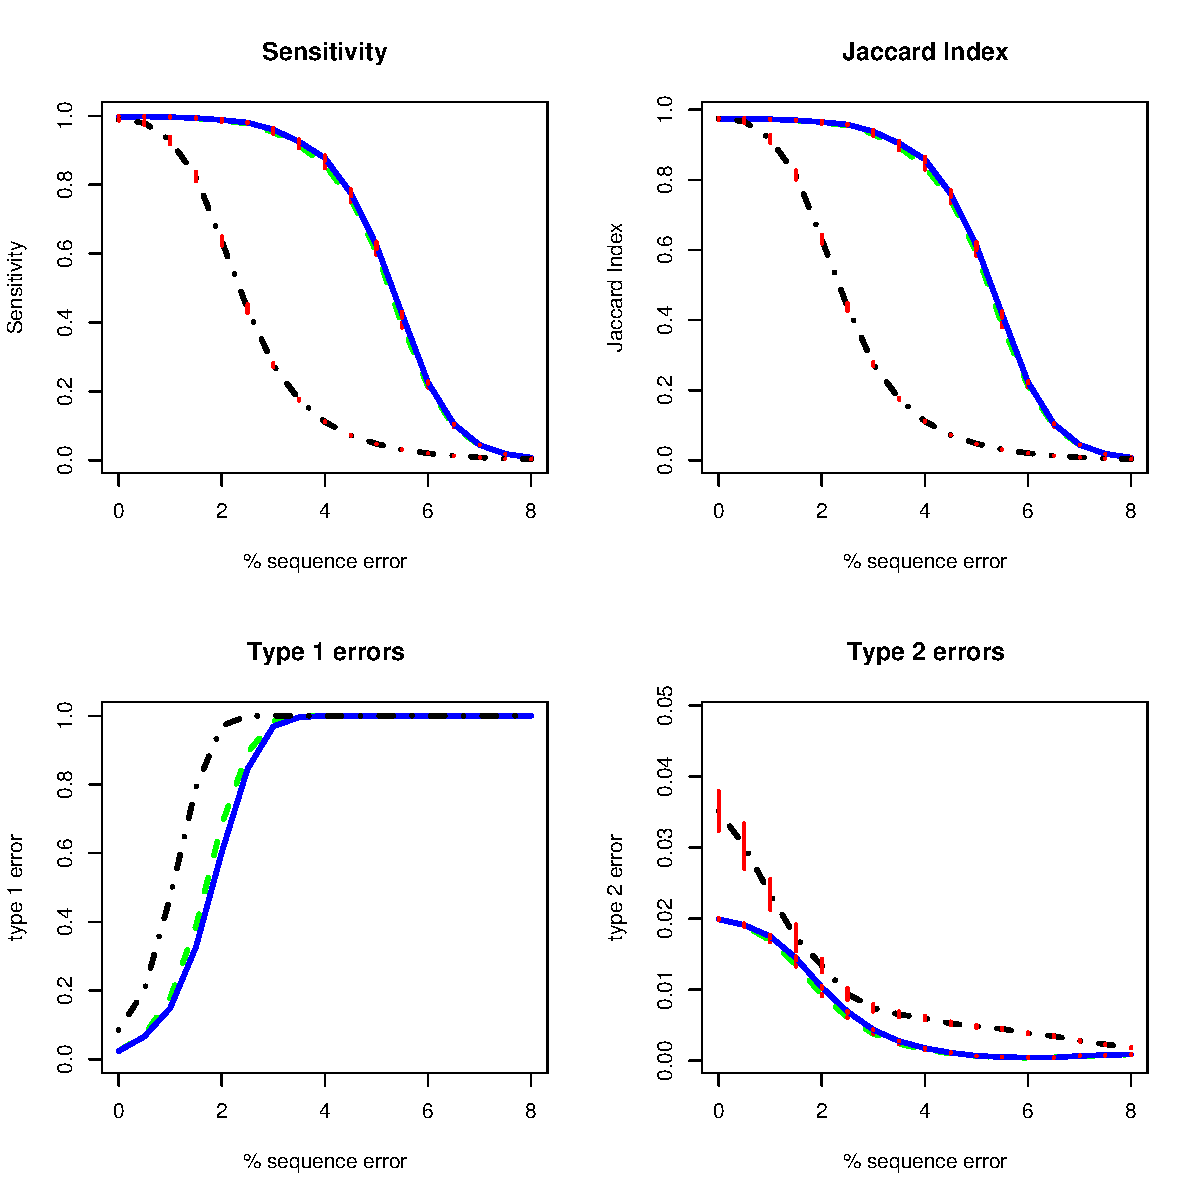
\includegraphics[width=3.35in]{pics.d/SeJiT1T2x40.pdf}}
  \caption{Comparisons of Sensitivity, Jaccard Index, Type 1 error and
    Type 1 error, based on the average over 30 simulated Sanger
    Sequence ESTs sets derived from 100 zebra fish genes (see
    Supplementary Materials, Section C, for more details).  Blue/Solid
    = \peace, Green/Dash = \wcd \mc{(version 0.5.1)}, Black/Dot-Dash =
    \capthree; vertical tics = 95\% confidence intervals on estimates.
    Intervals are not presented for Type 1 error due to the effective
    lack of variance.}\label{SeJiT1T2}
\end{figure}

\begin{figure}
   \centerline{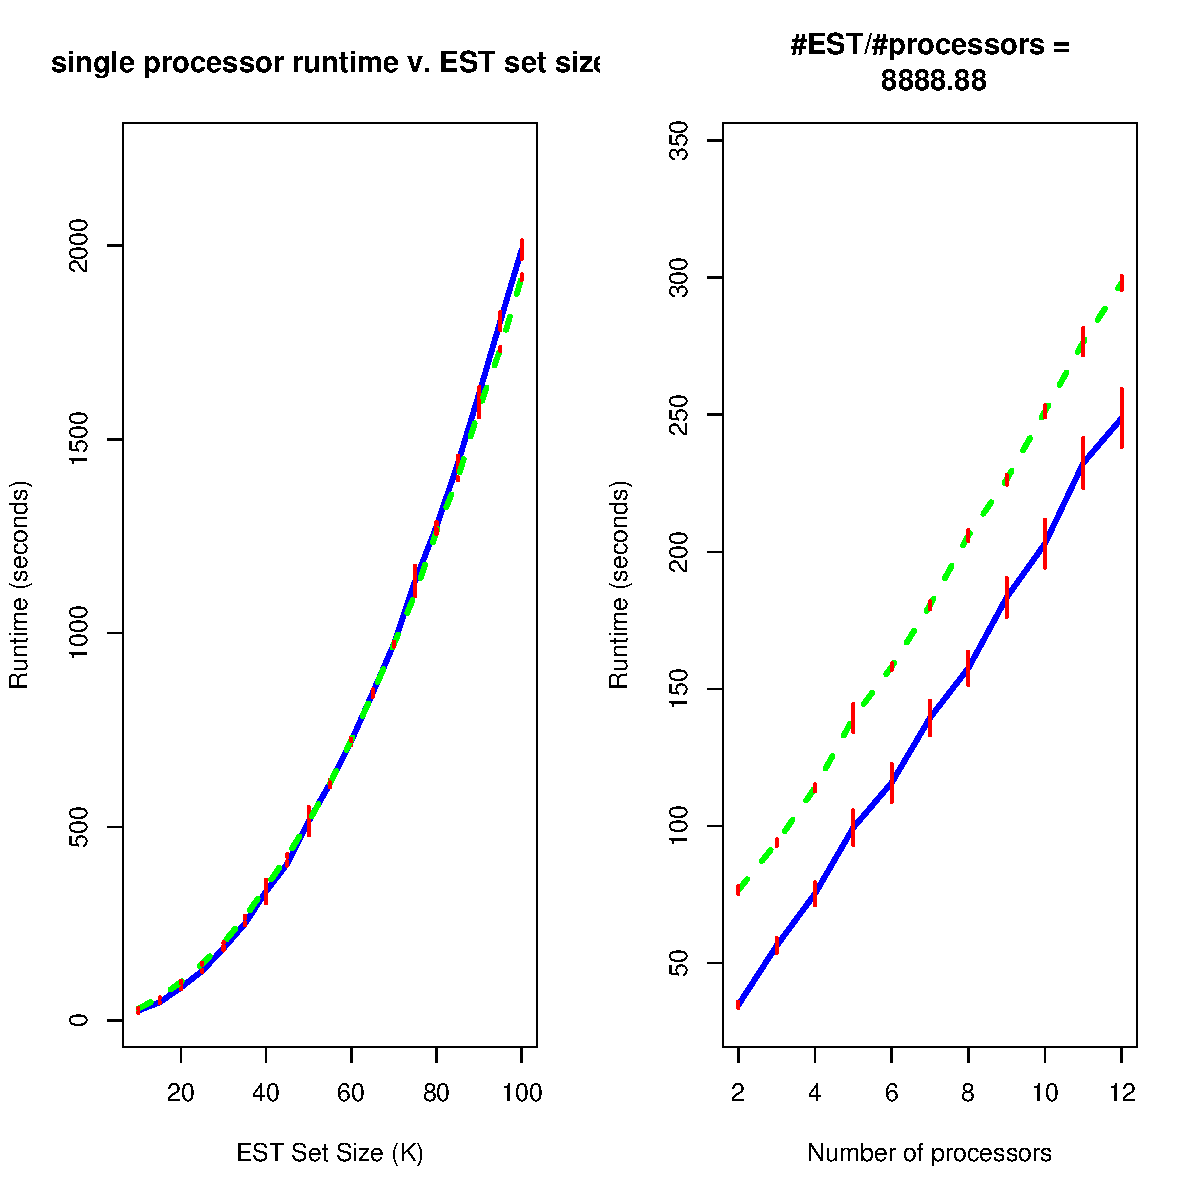
\includegraphics[width=3.35in]{pics.d/seq_parallel.pdf}}
   \caption{Comparisons of Runtime: On left, we compare the sequential
     runtime of \peace\/ (blue) and \wcd\/ (green) on simulate sets
     ranging in size from 10K sequences to 100K sequences.  (\capthree\/
     runtime is not reported, as the time spent on clustering cannot
     be differentiated from the time spent on assembly.)  On right,
     a comparison when run in parallel, ranging the number of
     processors from 2 to 12 while holding the EST/Processor ratio
     steady at the constant 8888.  All values represent the average
     of 30 runs; vertical tics = 95\% confidence intervals on
     estimates.  All runs were done on a 3.0 GHz Intel Xeon EM64T CPU with a 2 MB
     cache and 800 MHz front side bus, model number Xeon LV 3.0 (2005).}\label{seq_parallel}
\end{figure}

\mc{In applying the tools to real data Sanger data, we used the Human
Benchmark Data Set used to test \easycluster\/ \cite{Picardi09}, and
the A076941.fa {\it Arabidopsis thaliana} data set used to test WCD
\cite{Hazelhurst08a,Hazelhurst08b}, (see Table~\ref{SangerReal}).  We notice essentially identical
results for PEACE and WCD in quality, both significantly better than
Cap3 in Sensitivity and Type 1 error rate, while slightly worse in the
Jaccard Index and Type 2 error.  In runtime we see some inconsistency,
with PEACE showing a 60\% runtime improvement in the first data set,
but requiring 20\% more time in the Arabidopsis data set.  In Section~D.1
of the Supplementary Materials we present runtimes several more
sets, observing that while \peace\/ appears to be significantly more
faster on the smaller sets, \wcd\/ does overtake it for larger sets.}


\begin{table*}[tbp]
\begin{center}
\begin{tabular} {| c || c || c | c | c | c | c | c | c |}
\hline
 & 
& Sensitivity & Jaccard & \begin{tabular}{c} Type 1 \\
  error \end{tabular} & \begin{tabular}{c} Type 2 \\
  error \end{tabular} &
\begin{tabular}{c} Number \\ of  \\
    Clusters \end{tabular} & \begin{tabular}{c} Number \\ of \\
    Singletons \end{tabular}
    & \begin{tabular}{c} Single \\ processor \\ runtime (s) \end{tabular}\\
\hline
\hline Bicyclist Human & \peace & 0.998 & 0.672 & 0.153 & 0.042 & 118 & 21 & 293 \\
\cline{2-9} Benchmark & \wcd & 0.998 & 0.672 & 0.144 & 0.044 & 113 & 16 & 804 \\
\cline{2-9} (111 Genes) & \capthree & 0.657 & 0.643 & 1.000 & 0.001 & 2269 & 1827 & \mbox{NA} \\
\hline
\hline WCD A076941 & \peace & 0.932 & 0.475 & 0.351 & 0.027 & 18825 & 8951 & 1166\\
\cline{2-9} Benchmark & \wcd & 0.933 & 0.476 & 0.350 &  0.027 & 18787 & 8553 & 966 \\
\cline{2-9} (13240 genes) & \capthree & 0.826 & 0.802 & 0.486 & 0.014 & 25042 & 14916 &
\mbox{NA} \\
\hline
\end{tabular}
\end{center}
\caption{Comparisons of runs on the EasyCluster human Benchmark
  Data Set and the WCD A076941 Arabidopsis thaliana data set using the
  standard quality measurements.}\label{SangerReal}
\end{table*}


% we started with a set of
% approximately $190,000$ clean Sanger ESTs derived from the {\it
%   Chlamydomonas reinhardtii} genome \cite{Liang2008}.  To compute
% sensitivity we used the {\it gmap} tool \cite{Wu05} to map the
% fragment set to the genome, taking this as our reference clustering.
% We see slight improvements in \peace\/ over \wcd\/ in both sensitivity
% and Type 1 error (both significantly outperforming \capthree).  Using
% the \mc{Arabidopsis} data set used in Hazelhurst {\it et al.}
% \cite{Hazelhurst08a} \peace\/ again shows slight improvements in
% sensitivity and Type 1 error rates, with an 18\% speedup for \peace\/ 
% (see Supplementary Materials, Section~D, for more details).

\mc{We tested the three tools on short-read data using the \metasim\/
  tool of {\it Richter et al.} \cite{Richter2008}.  Encoded into
  \metasim\/ are sequence generation and error models corresponding to
  several technologies, including the 454 short-read technology.
  Leaving \capthree\/ and \wcd\/ at their default values, but
  employing the {\it adaptive $d^2$} strategy for short read sequences
  (see Section~C in the supplementary materials), we find a that
  \peace\/ performs significantly better than the other two tools on
  454 data using the default \metasim\/ model (with sequence sizes
  ranging in size from 200bp to 370bp, at an average size of 250bp and
  a standard deviation of 17bp).  Over thirty runs, we see an average
  sensitivity 0.884 for \peace, 0.331\/ for \wcd, and 0.004 for
  \capthree.  For the Jaccard Index we get essentially the same
  numbers.  For 100 transcript \peace\/ creates 128 clusters (as
  opposed to 6,370 and 19245 clusters for \wcd\/ and \capthree), and
  creates only 3 singletons (as opposed to 5,850 and 15432).  We do
  note that it is likely that the \wcd results could be considerably
  improved by the adjustment of a few parameters, but were unable to
  determine how to do that.  (Runtime of \peace\/ was somewhat slower
  than that of \wcd, but given the significant improvement in quality
  of results this is unimportant.)}

\section{Conclusions}

\mc{Here we have presented \peace, a stand alone tool for the
high-throughput clustering of transcript fragments capable of dealing
with sequences as short as 50 bases.  \peace\/, available at
\href{http://www.peace-tools.org}{www.peace-tools.org}, is open-source
and managed through a user friendly GUI that enables both local and
remote installation and execution in sequential or parallel mode.
Based on a novel algorithm for the clustering of the fragments by gene
association, \peace\/ shows significant improvement in sensitivity,
over the competing \wcd\/ tool \cite{Hazelhurst08a} when applied to
NGS reads, matches \wcd\/ when applied to Traditional Sanger
Sequencing output, and shows an order of magnitude in improvement over
the clustering performed in the course of assembly by the \capthree\/
tool \cite{Huang99}.}

As a clustering tool based on sequence distance, \peace\/ faces
certain inherent limitations. For example, \peace\/ cannot handle
duplicate genes; like \wcd\/, it is unable to separate clusters
corresponding to genes with a greater than 88\% similarity.
Similarly, other natural biological effects (e.g. the trans-splicing of
transcripts), effects from poorly cleaned transcript data (e.g. the
failure to remove sequencing adapters or post-transcriptional
poly(A)/(T) tails), and the presence of low-complexity repeats can
cause similar effects in these clustering tools.  The problems can be
handled through the application of the assembler, and the ability to
apply any assembler to small cluster (as opposed to the data set as a
whole) results in a significant reduction in overall assembly time.

\section{Acknowledgements}

Dr. Karro was funded under a PhRMA Foundation Informatics Research
Starters Grant while conducting this research.  We would also like to
acknowledge Iddo Friedberg, David Woods, Elizabeth Bikun, Jens Mueller and David
Scoville at Miami University for their help with this project.

\vspace{3mm}
% Bib TeX

\bibliography{peace.bib}



\end{document}


% LocalWords:  arallel nalysis lustering ngine Rao Moler Ozden Zhang Liang ESTs
% LocalWords:  Karro XXXXX transcriptome pre isoforms SNPs unsequenced runtime
% LocalWords:  chlamydomondomonas ESTate PaCE xsact CLU WCD Hazelhurst et al th
% LocalWords:  CHUN nalyzer Prim's MSTs subgraph MPI SourceCode ESTSim runtimes
% LocalWords:  ests Chlamydomonas Reihartdii gmap CDNA transcriptomes cDNA www
% LocalWords:  reinhartdii conifergdb DNAc bp wcd reinhardtii PhRMA Iddo fasta
% LocalWords:  Friedberg Scoville OpenMPI initio multi Screenshots nvironment
% LocalWords:  ssembly xpression GenBank dbEST pyrosequencing ESTsim sim mRNAs
% LocalWords:  NGS polyA set's GHz Xeon Bikun Arabidopsis JVM Jaccard LV GUI's
% LocalWords:  Data Set thaliana data set EasyCluster MetaSim
